\chapter{Observing at the Marion Island Site}

Observing at the Marion Island site comes with consequences that need to be addressed. Those factors mainly affect the low-frequency experiments (\prizm / \albatros) discussed in this thesis, and they include RF quietness, ionospheric conditions, accessibility, and ability to support long baselines. Low-frequency observations require high angular resolution to improve the experiment's sensitivity. Systematics discussed in \S\ref{s:chall} widely dominate the experiments operating at frequencies $<$\SI{200}{MHz}. RFI from the frequency modulation (FM) transmitters is a substantial contributor in the low-frequency regime; thus, FM contamination is widespread into observation bands. Observing from remote deployment sites is a solution to the FM band contamination issue. Before site selection and deployment, radio environments must match the specific instrument's requirements when assessed. Accessibility is a common challenge that arises from remote site selection. Therefore, choosing a good observing location is generally a balance between	accessibility and radio-quietness. 

Marion Island was chosen as the observing site for \prizm\ and \albatros\ after evaluating the mentioned factors. Marion Island is the exceptionally radio-quiet environment for low-frequency observations, although the site is only accessible annually. The next section discusses the location in more detail.

\section{Marion Island}

Marion Island is a research base that forms part of the Prince Edward Islands shown in Figure~\ref{fig:marion}, located in the southern Indian Ocean at \ang{46;54;45}S, \ang{37;44;37}E. The South African National Antarctic Programme (SANAP) and the South African Department of Environmental Affairs (DEA) operate the research base shown in Figure~\ref{fig:base}. The island is $\sim$ \SI{2000}{\kilo\metre} from the nearest continental landmasses, has an area of 290~km$^2$, and the main base is positioned on the northeast side. Marion Island has a volcanic origin, and the terrain is scattered with many secondary craters and small lakes. There are abundant snow and rain, and the vegetation is mainly mosses and ferns. The lowland regions are marshy due to high precipitation. It is incredibly windy and mostly cloudy throughout the year.

\begin{figure}
	\centering
	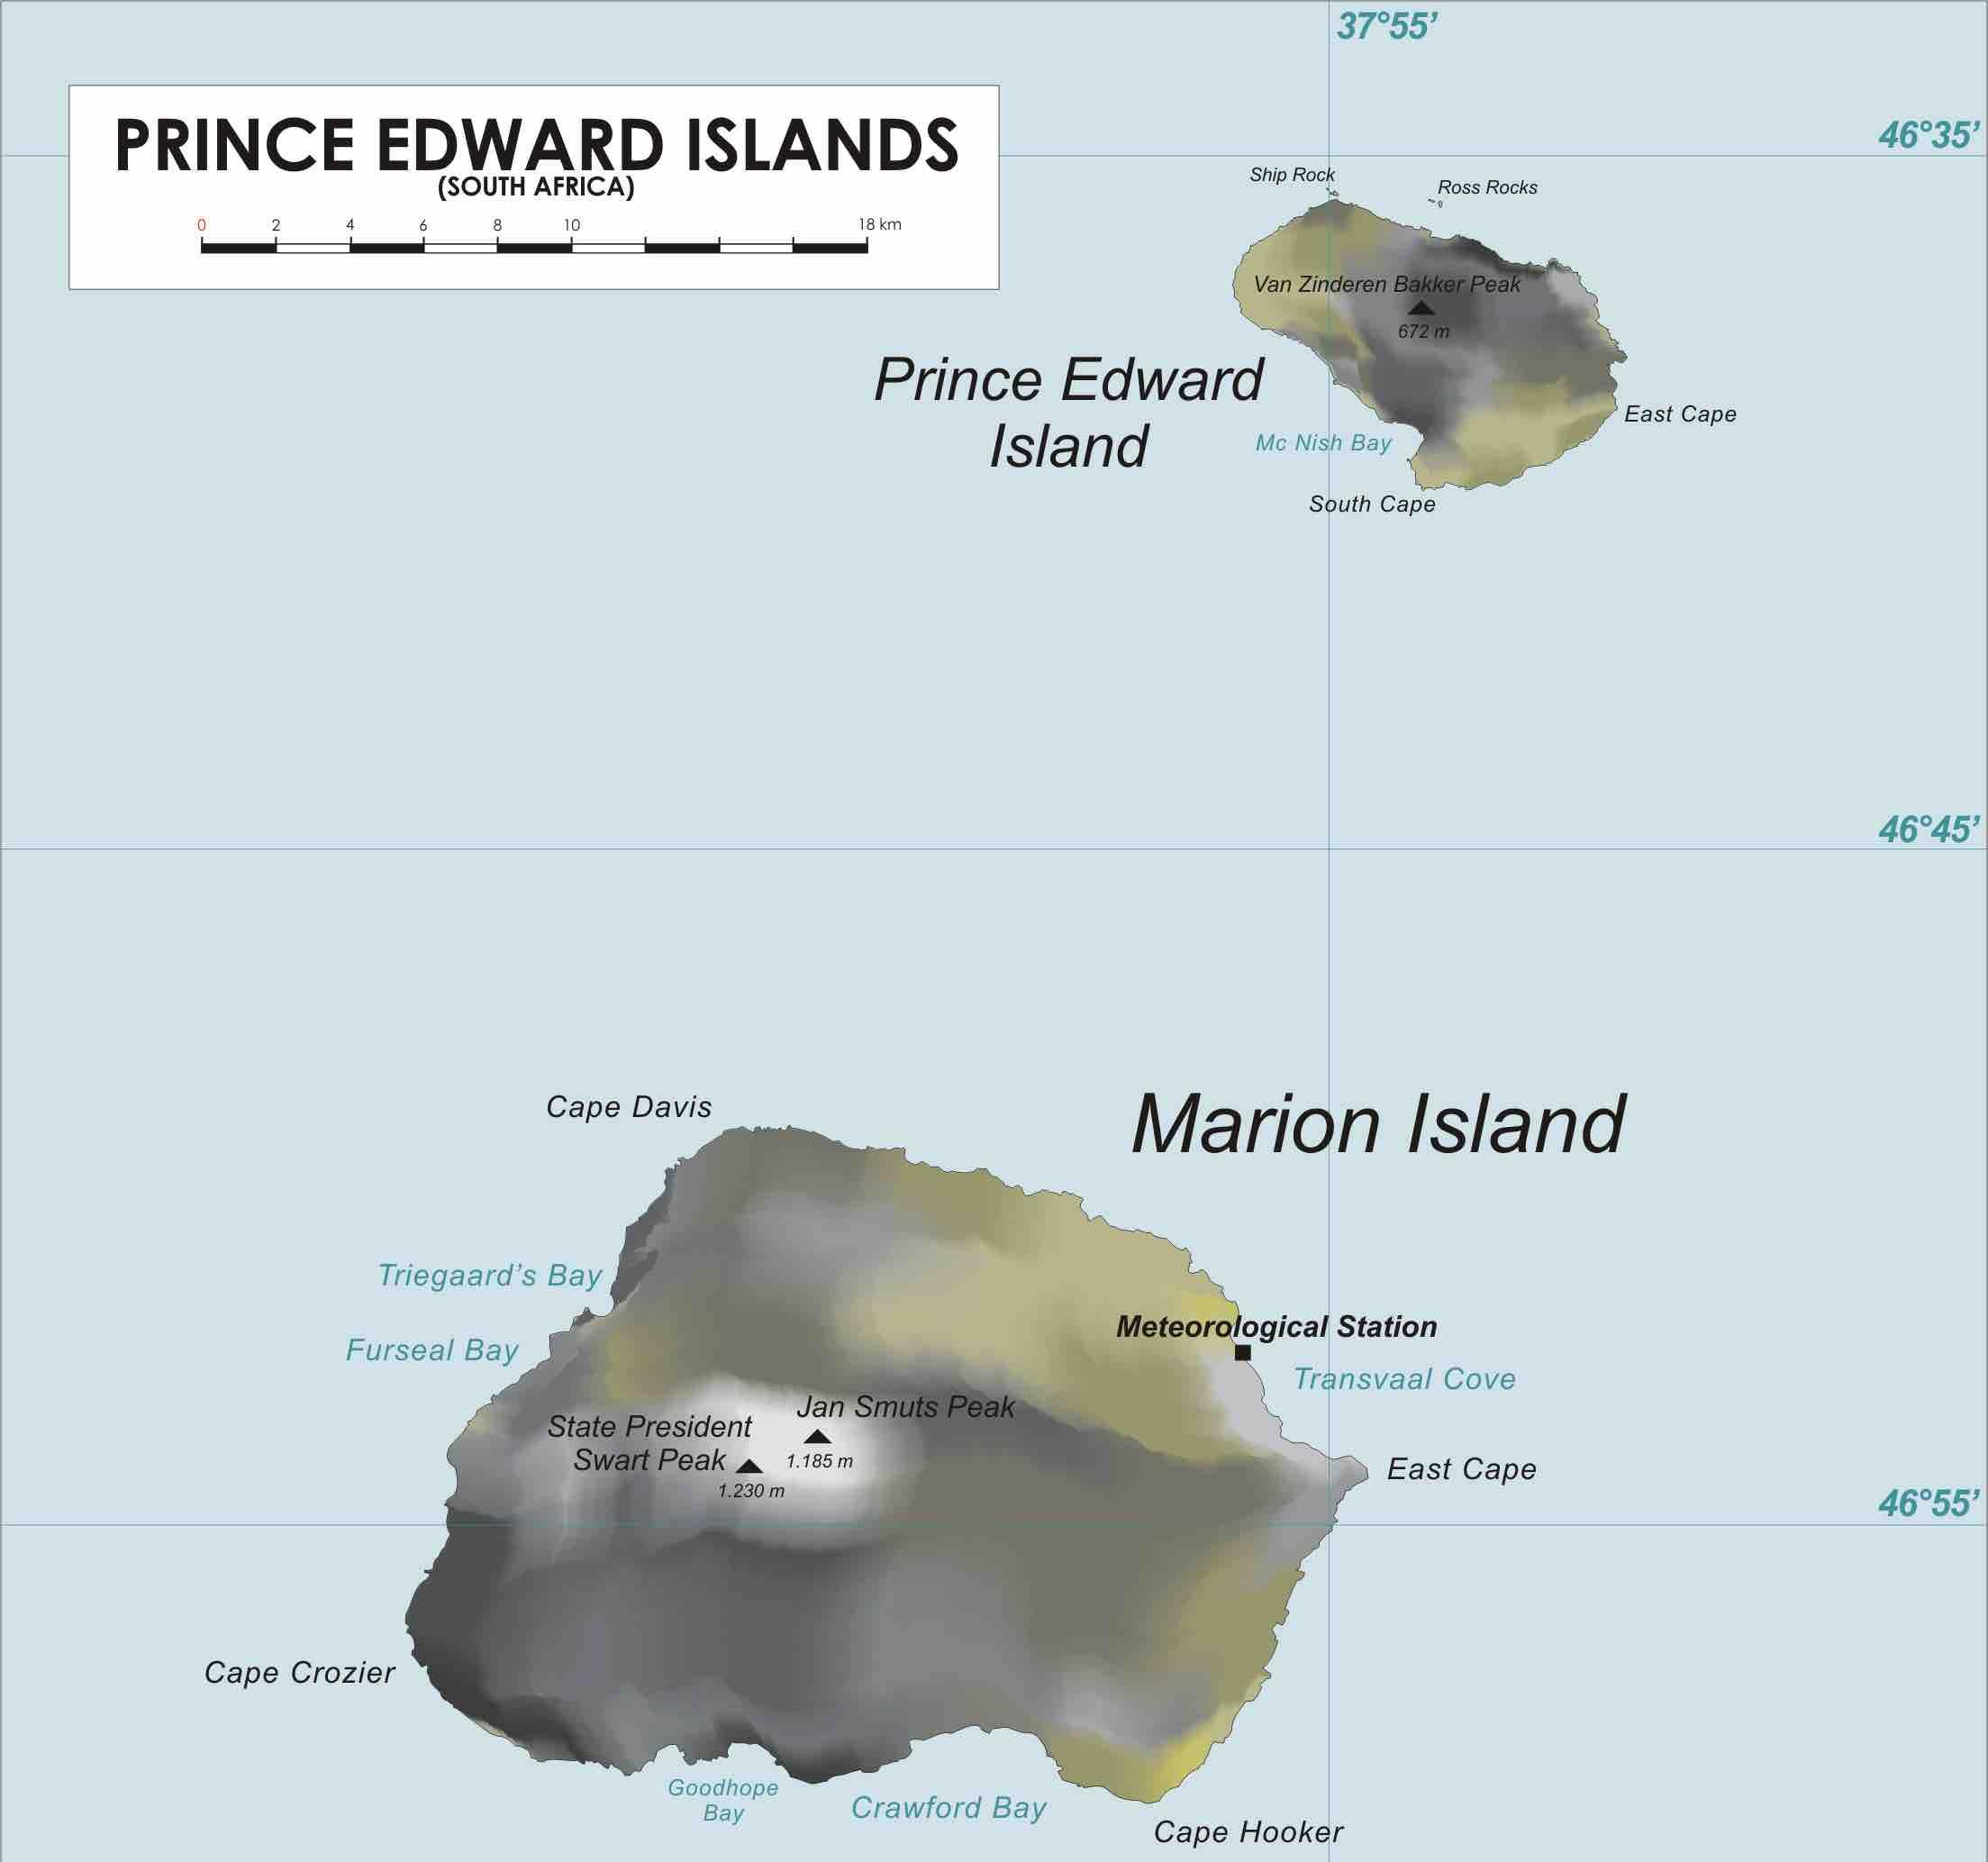
\includegraphics[width=\linewidth]{Figures/marion}
	\caption{The two islands in the Prince Edward Islands are Prince Edward Island and Marion Island, located in the sub-Antarctic Indian ocean~\citep{PEI}}.
	\label{fig:marion}
\end{figure}

\begin{figure}
	\centering
	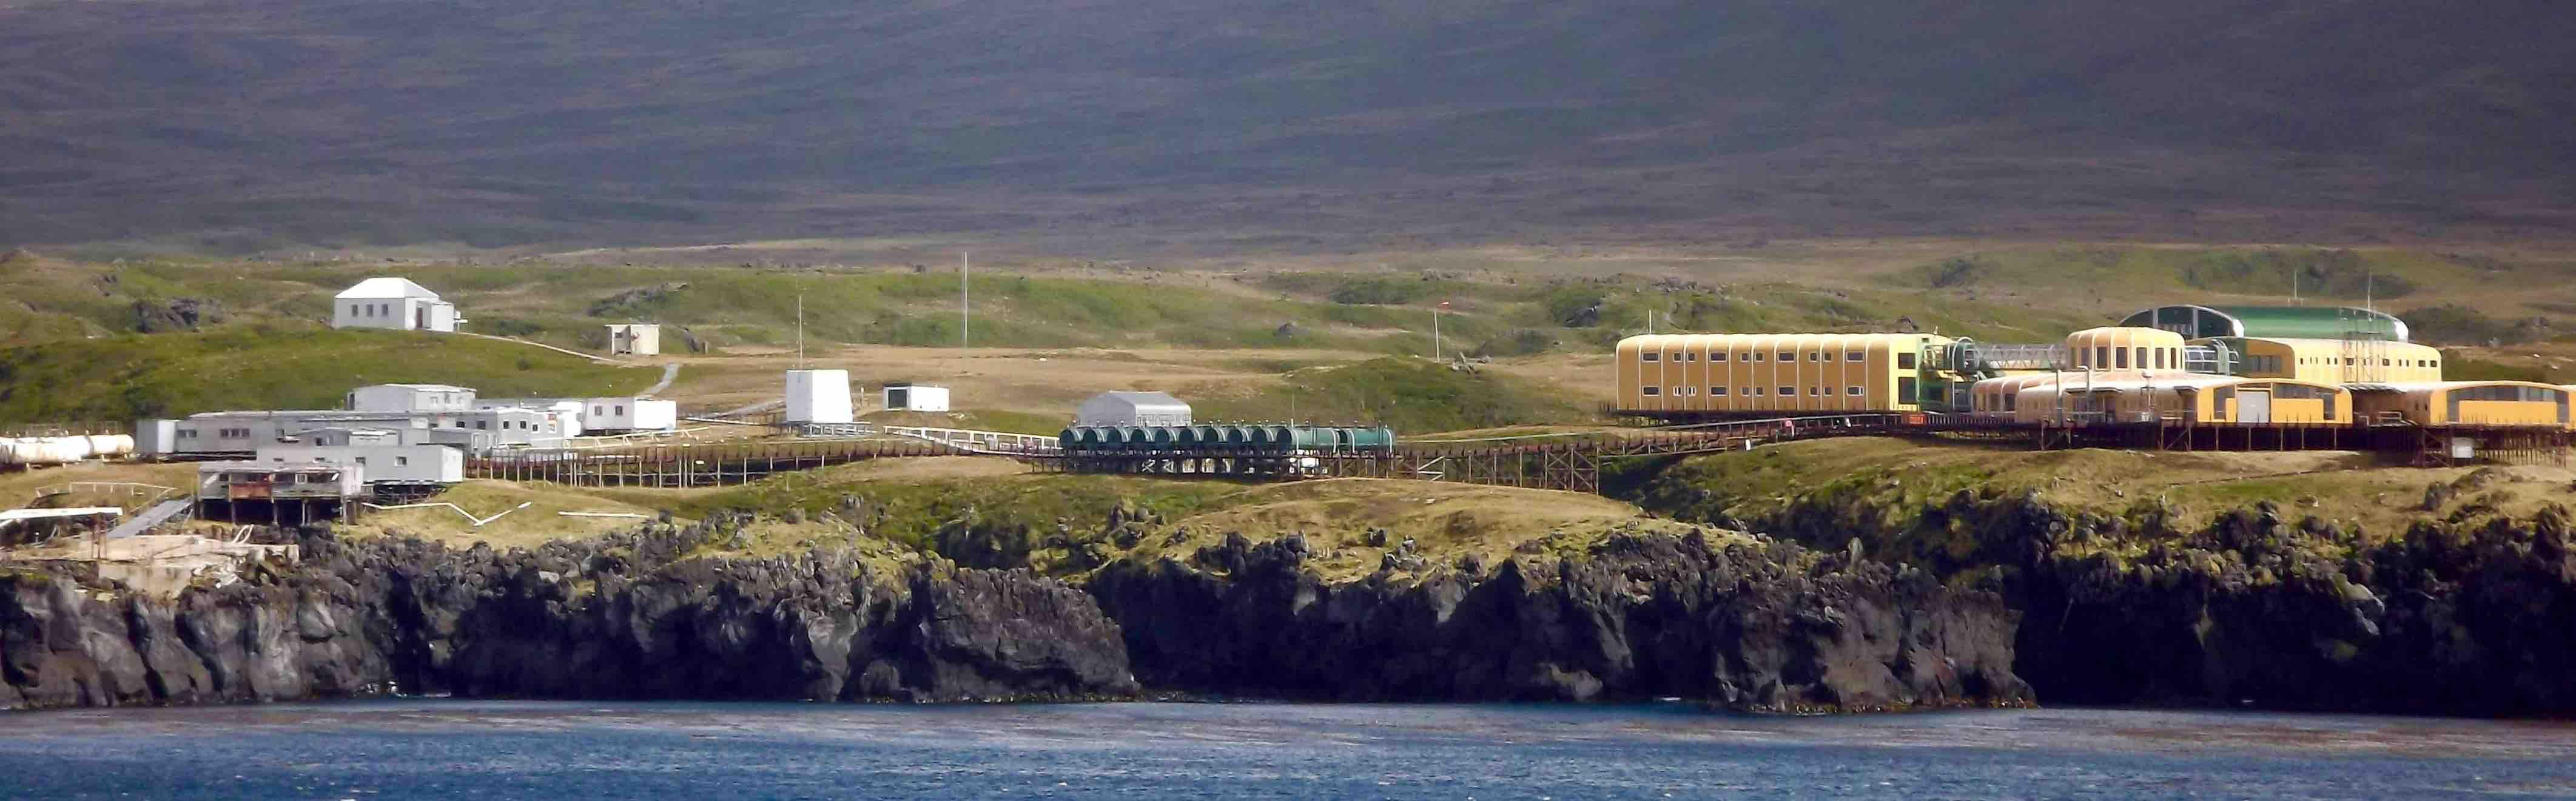
\includegraphics[width=\linewidth]{Figures/base}
	\caption{Marion Island new (yellow buildings) and old base (white buildings). The green building partially visible behind the new base is the emergency base that serves as a helipad and a hangar for helicopter operations.}
	\label{fig:base}
\end{figure}

The DEA owns the S. A. Agulhas II \footnote{\url{https://en.wikipedia.org/wiki/S. A. Agulhas II}}, a South African ice-breaking polar supply and research ship that services the island every year in April. During the relief voyage in April, three weeks are spent on the island deploying and maintaining instruments. Marion Island has been traditionally used for the research fields of space weather, geology, meteorology, mammalogy, ornithology, and botany. The main Marion base accommodates all the researchers participating in the relief voyage and overwintering team members. Figure~\ref{fig:site} shows the nine rest huts (Kildalkey, Watertunnel, Cape Davis, Grey-headed, Mixed Pickle, Repettos, Rooks, Swartkops, and, Katedraal) that researchers use while traversing the island. The \prizm\ instrument was deployed \SI{4}{\kilo \meter} southwest of the main base (\ang{46;53;13}S, \ang{37;49;10.7}E) as the first radio astronomy experiment in Marion Island, followed by the \albatros\ pathfinder instruments on the same site. 

\begin{figure}
	\centering
	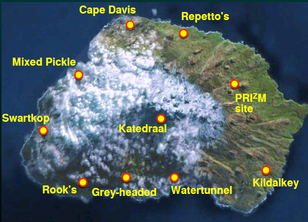
\includegraphics[width=\linewidth]{Figures/site}
	\caption{Marion Island rest huts and the \prizm\ site where the first radio astronomy instrument was deployed and subsequently \albatros\ pathfinder.}
	\label{fig:site}
\end{figure}

\section{Advantages of Observing from Marion Island}

This section presents a brief overview of the site selection process on Marion, and a full description is available in~\citet{2019JAI.....850004P}. In choosing the observing site for \prizm\ and \albatros, several radio spectrum measurements were done on different sites, including the South African Karoo desert. The radio-quiet environment of Marion Island surpasses that of the South African Karoo desert, as shown in Figure~\ref{fig:karoo}. At Marion Island, there is no evident detection of RFI contamination in the FM band, and the only significant RFI visible within the PRIZM operating range is Orbcomm satellite transmission at \SIrange{137}{138}{\mega\hertz} and the \SI{250}{\mega\hertz} FPGA clock artifact visible at \SI{125}{\mega\hertz}. The enhanced RFI from meteor scattering is a common phenomenon in several remote sites excluding Marion Island, as there have not been evident measurements of such RFI. At a speed of $\sim$ \SIrange{10}{75}{\kilo \meter \per \second}, meteoroids enter the Earth's atmosphere, and contact with the atmosphere results in the air molecules ionization. During this time, by bouncing radio waves off the ionized trail, brief contact paths can be formed between radio stations several thousand miles away from each other. Likewise, terrestrial RFI sometimes gets scattered off the trail over long distances. Depending on the meteor trail's location and the intensity of meteor activity, the magnitude of RFI due to meteor dispersion varies~\citep{1996pimo.conf...99W}.

\begin{figure}
	\centering
	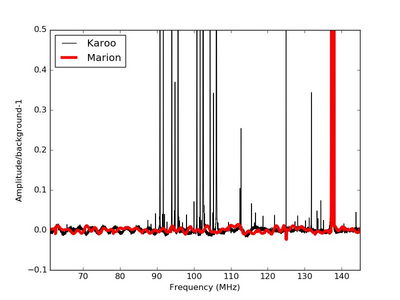
\includegraphics[width=\linewidth]{Figures/karoo}
	\caption{Comparison of radio spectrum on Marion (thick red) and in the Karoo desert (thin black). The fractional amplitude above a background fit the raw and uncalibrated data without RFI excision. Orbcomm satellite transmission is visible at 137–138 MHz; there is no visible RFI in Marion's data. The feature at 125 MHz is an artifact of the 250 MHz FPGA clock and not due to RFI~\citep{2019JAI.....850004P}}
	\label{fig:karoo}
\end{figure}

Figure~\ref{fig:rfi} shows the RFI spectrum comparison between the \prizm\ deployment site \SI{4}{\kilo\metre} away from the island's main base. The selection of \prizm\ site was based on having a reasonably dry and even terrain, i.e., not in a mire, a reasonable hiking distance from the main base, and keeping the locally generated RFI at its minimum. Locally generated RFI less impacts the \prizm\ site Junior's Kop situated between the deployment site and the island's main base provides enhanced RFI shielding of \SI{\sim60}{\decibel}. The reduction in power arises from a physical distance from the base and the landmass in Junior's kop. The helicopter was operating near the base when the RFI measurements were taken and transmitting at a frequency of \SI{123.45}{\mega\hertz}. The helicopter's transmission line was an unexpected origin of RFI that enabled the calibration of the relative levels at Junior's kop vs. the main base.

\begin{figure}
	\centering
	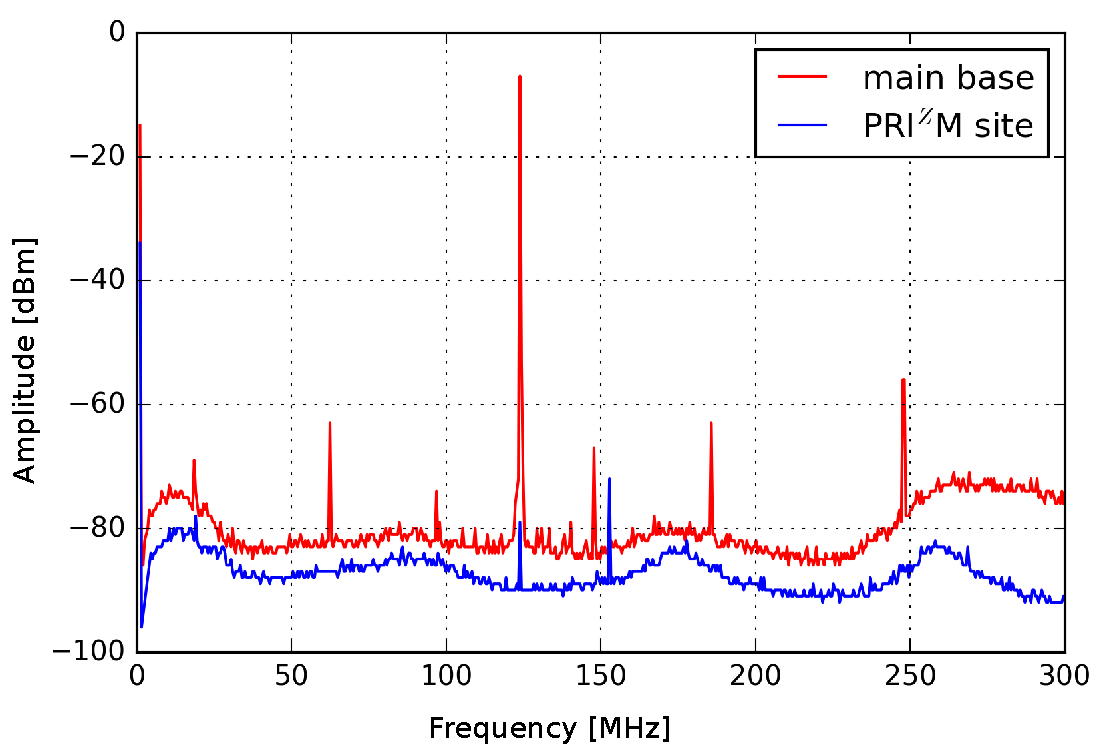
\includegraphics[width=\linewidth]{Figures/rfi}
	\caption{RFI measurement differentiated from the Marion base and the \prizm observing site. When the measurements were taken, the spectrum analyzer was set to max hold, and the measurement period coincided with the helicopter's operation near the base and transmitting at \SI{123.45}{\mega\hertz}. A rough benchmark of $\sim$60 dB signal suppression in received power at both locations arising from a combination of attenuation from Junior's kop and the distance between the \prizm site and the base. The peak at 156 MHz is a transmission from a handheld radio~\citep{2019JAI.....850004P}.}
	\label{fig:rfi}
\end{figure}

Figure~\ref{fig:IRI_model} shows the international reference ionosphere (IRI) model~\citep{ars-16-1-2018} predictions illustrating the minimum ionospheric plasma cutoff frequency during the last solar minima. The development of new low-frequency experiments is predominantly driven by the lack of knowledge of what lies in the sky at frequencies $\lessapprox$\SI{30}{\mega\hertz}.  According to the international reference ionospheric (IRI) model prediction, measurements of the sky at $\lessapprox$\SI{30}{\mega\hertz} do not look entirely impossible because, during the last solar minimum, the ionospheric plasma cutoff frequency was predicted to be $\sim$\SI{1.5}{\mega\hertz} at Marion Island. Since another solar minimum is being experienced~\citep{2018NatCo...9.5209B}, it is an excellent opportunity to develop and implement new low-frequency observations. The prediction shows Marion Island, Dome C in Antarctica, and Hobart in Tasmania, where Reber performed his \SI{2}{\mega\hertz} observation. They have the potential to provide new views of the Earth's ionosphere, which absorbs and refracts at radio frequencies and becomes utterly opaque below the plasma cutoff frequency. 

The total Marion takeover voyage period is $\sim$ one and a half months. This period is further shortened by the days it takes to and from the island, the weather, and logistical delays. The site is entirely inaccessible on days with gale-force winds (roaring forties)—the sun sets early, limiting the daylight and more extended access to the instruments. The site's path is riddled with lava rocks and secret mires, rendering the trek incredibly difficult. Furthermore, the island is an environmentally protected area that sets the boundaries on equipment installations. Although it is a pretty steep price to pay, the reward is an exceptional RF-quiet environment. In the next two chapters, the \prizm\ and \albatros\ experiments are discussed in detail.

\begin{figure}
	\centering
	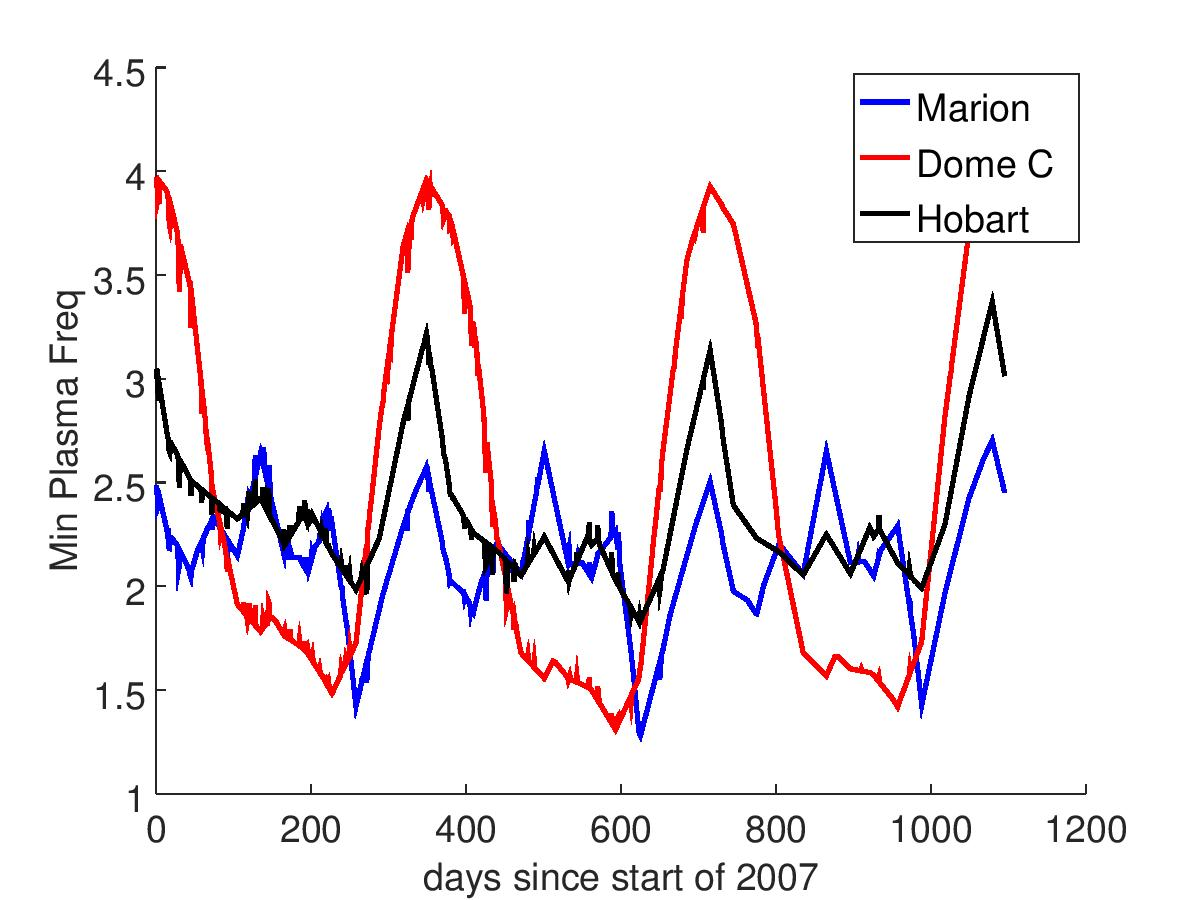
\includegraphics[width=\linewidth]{Figures/IRI_model}
	\caption{The International Reference Ionosphere model predictions illustrating the minimum ionospheric plasma cutoff frequency during last solar minima. At Marion Island, Dome C in Antarctica and Hobart in Tasmania the plasma frequency may drop as low as $\sim$\SI{1.5}{\mega\hertz}~\citep{2020arXiv200812208C}.}
	\label{fig:IRI_model}
\end{figure}
